\subsection{Разработка аппаратной части комплекса}

Для управления светодиодной лентой, необходима генерация ШИМ-сигнала, подаваемая на контакт Din светодиодной ленты. Это, в свою очередь накладывает свои требования к генератору ШИМ-сигнала.

Для передачи информации, на контакт Din светодиодной ленты должны поступать последовательности по 24 бита, или по 3 байта, которые отвечают за цвет определённого светодиода. При модуляции используются длительности импульсов, согласно таблице~\ref{tab:ws2812__data_transfer_time}~\cite{Worldseim}.

\begin{table}[H]
  \caption{Длительность импульсов для управления светодиодом WS2812b}
  \label{tab:ws2812__data_transfer_time}
  \begin{tabular}{|c|l|c|}
  \hline
  \textbf{Обозначение} & \multicolumn{1}{c|}{\textbf{Описание}} & \textbf{Время} \\ \hline
  T0H                  & код "0", время высокого уровня         & 0,35 мкс       \\ \hline
  T1H                  & код "1", время высокого уровня         & 0,9 мкс        \\ \hline
  T0L                  & код "0", время низкого уровня          & 0,9 мкс        \\ \hline
  T1L                  & код "1", время низкого уровня          & 0,35 мкс       \\ \hline
  RES                  & время низкого уровня                   & 50 мкс         \\ \hline
  \end{tabular}
\end{table}

Визуально ШИМ импульсы представлены на рисунке~\ref{img:WS2812__PWM_codes}.

\begin{figure}[H]
  \centering
  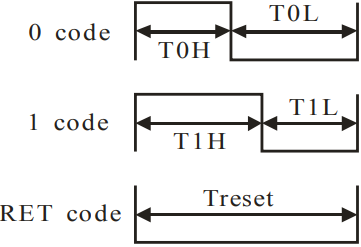
\includegraphics[height=0.2\textheight]{assets/images/practical/PWM__codes.png}
  \caption{ШИМ импульсы для управления WS2812b}
  \label{img:WS2812__PWM_codes}
\end{figure}

При кодировании цвета светодиода, последовательность из 24 бит представляется как 3 подряд идущих пакета, описывающих определённый основной сигнал. Первый пакет описывает зелёную составляющую цвета, второй --- красную, третий --- синюю. Биты в пакетах идут от старшего к младшему.

Например, для описания цвета, представленного в RGB как (18, 88, 160), необходимо преобразовать его в GRB, (88, 18, 160). Затем перевести их в двоичный вид, 01011000 00010010 10100000, и подать на вход Din светодиодной ленты в ШИМ. Для данного примера, ШИМ будет выглядеть как на рисунке~\ref{img:WS2812__PWM_example}.

\begin{figure}[H]
  \centering
  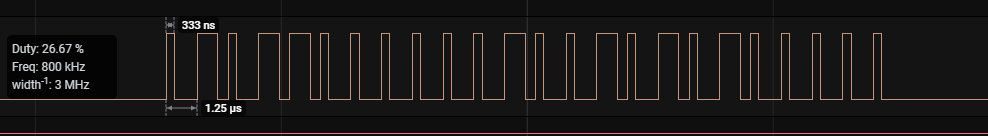
\includegraphics[width=0.9\textwidth]{assets/images/practical/PWM__example.jpg}
  \caption{Пример ШИМ для кодирования цвета}
  \label{img:WS2812__PWM_example}
\end{figure}

Для генерации ШИМ можно использовать расположенные на плате Raspberry Pi GPIO контакты.

Для программной генерации ШИМ можно использовать все контакты GPIO, но при таком подходе часть аппаратных ресурсов платформы будет тратиться на генерацию и кодирование импульсов, что влечёт за собой уменьшение производительности всей системы. Для аппаратной генерации ШИМ предназначены контакты GPIO12, GPIO13, GPIO18, GPIO19 Raspberry Pi. В этом случае достигается большая производительность системы и упрощение для разработчика при работе с напряжением на контактах GPIO. Полная карта контактов Raspberry Pi представлена на рисунке~\ref{img:raspberrypi__GPIO_pinout_diagram}.

\begin{figure}[H]
  \centering
  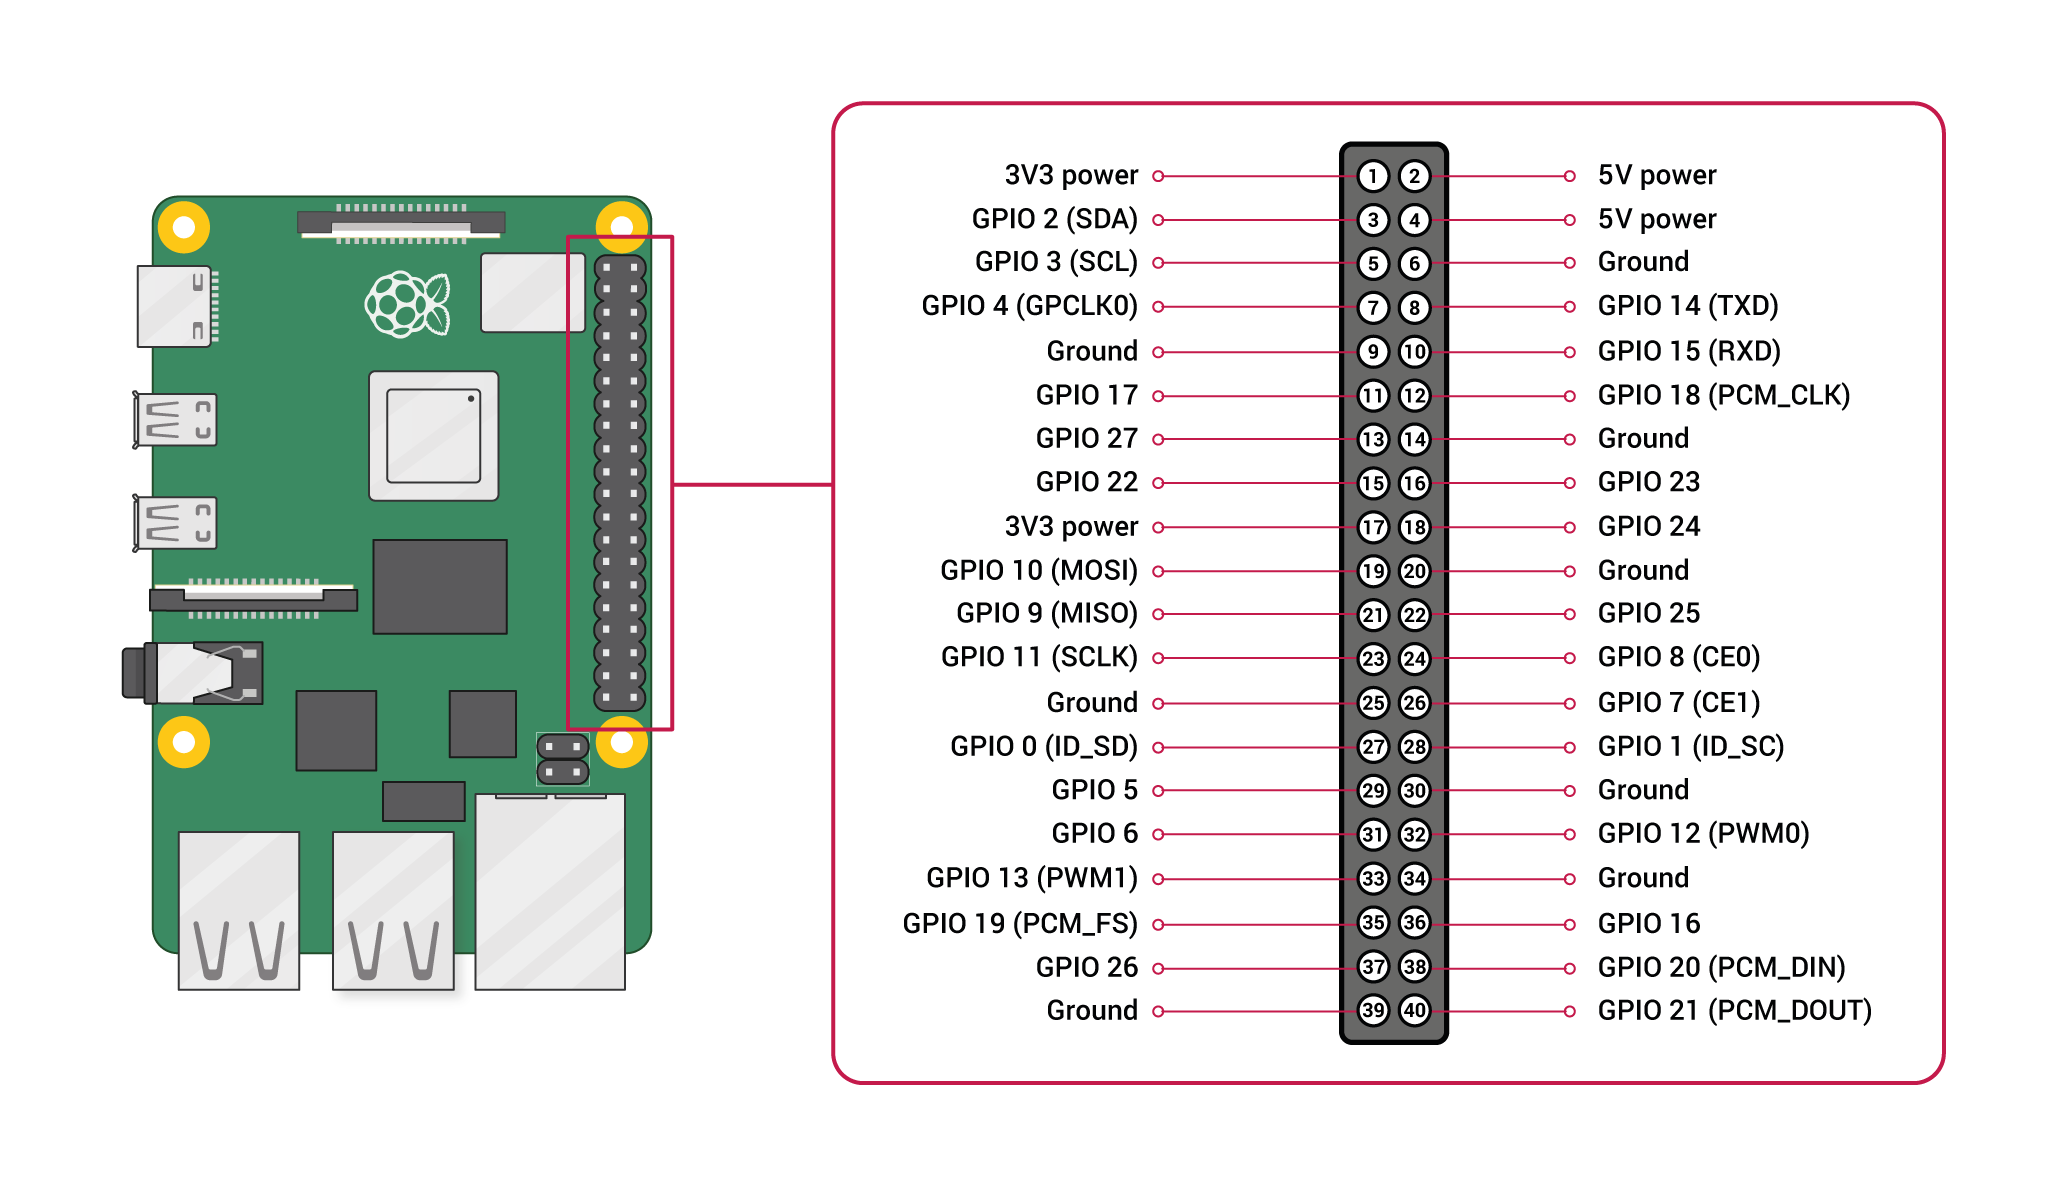
\includegraphics[width=0.9\textwidth]{assets/images/practical/GPIO-Pinout-Diagram.png}
  \caption{Карта GPIO контактов Raspberry Pi}
  \label{img:raspberrypi__GPIO_pinout_diagram}
\end{figure}

Ввиду этого для генерации ШИМ был выбран контакт GPIO18, обозначен номером 12 на карте~\ref{img:raspberrypi__GPIO_pinout_diagram}. Также, согласно карте GPIO контактов, в качестве контакта заземления был выбран контакт 6.

В следствие этого, был разработан итоговый макет программно-аппаратного комплекса. Макет представлен на рисунке~\ref{img:all__schema}.

\begin{figure}[H]
  \centering
  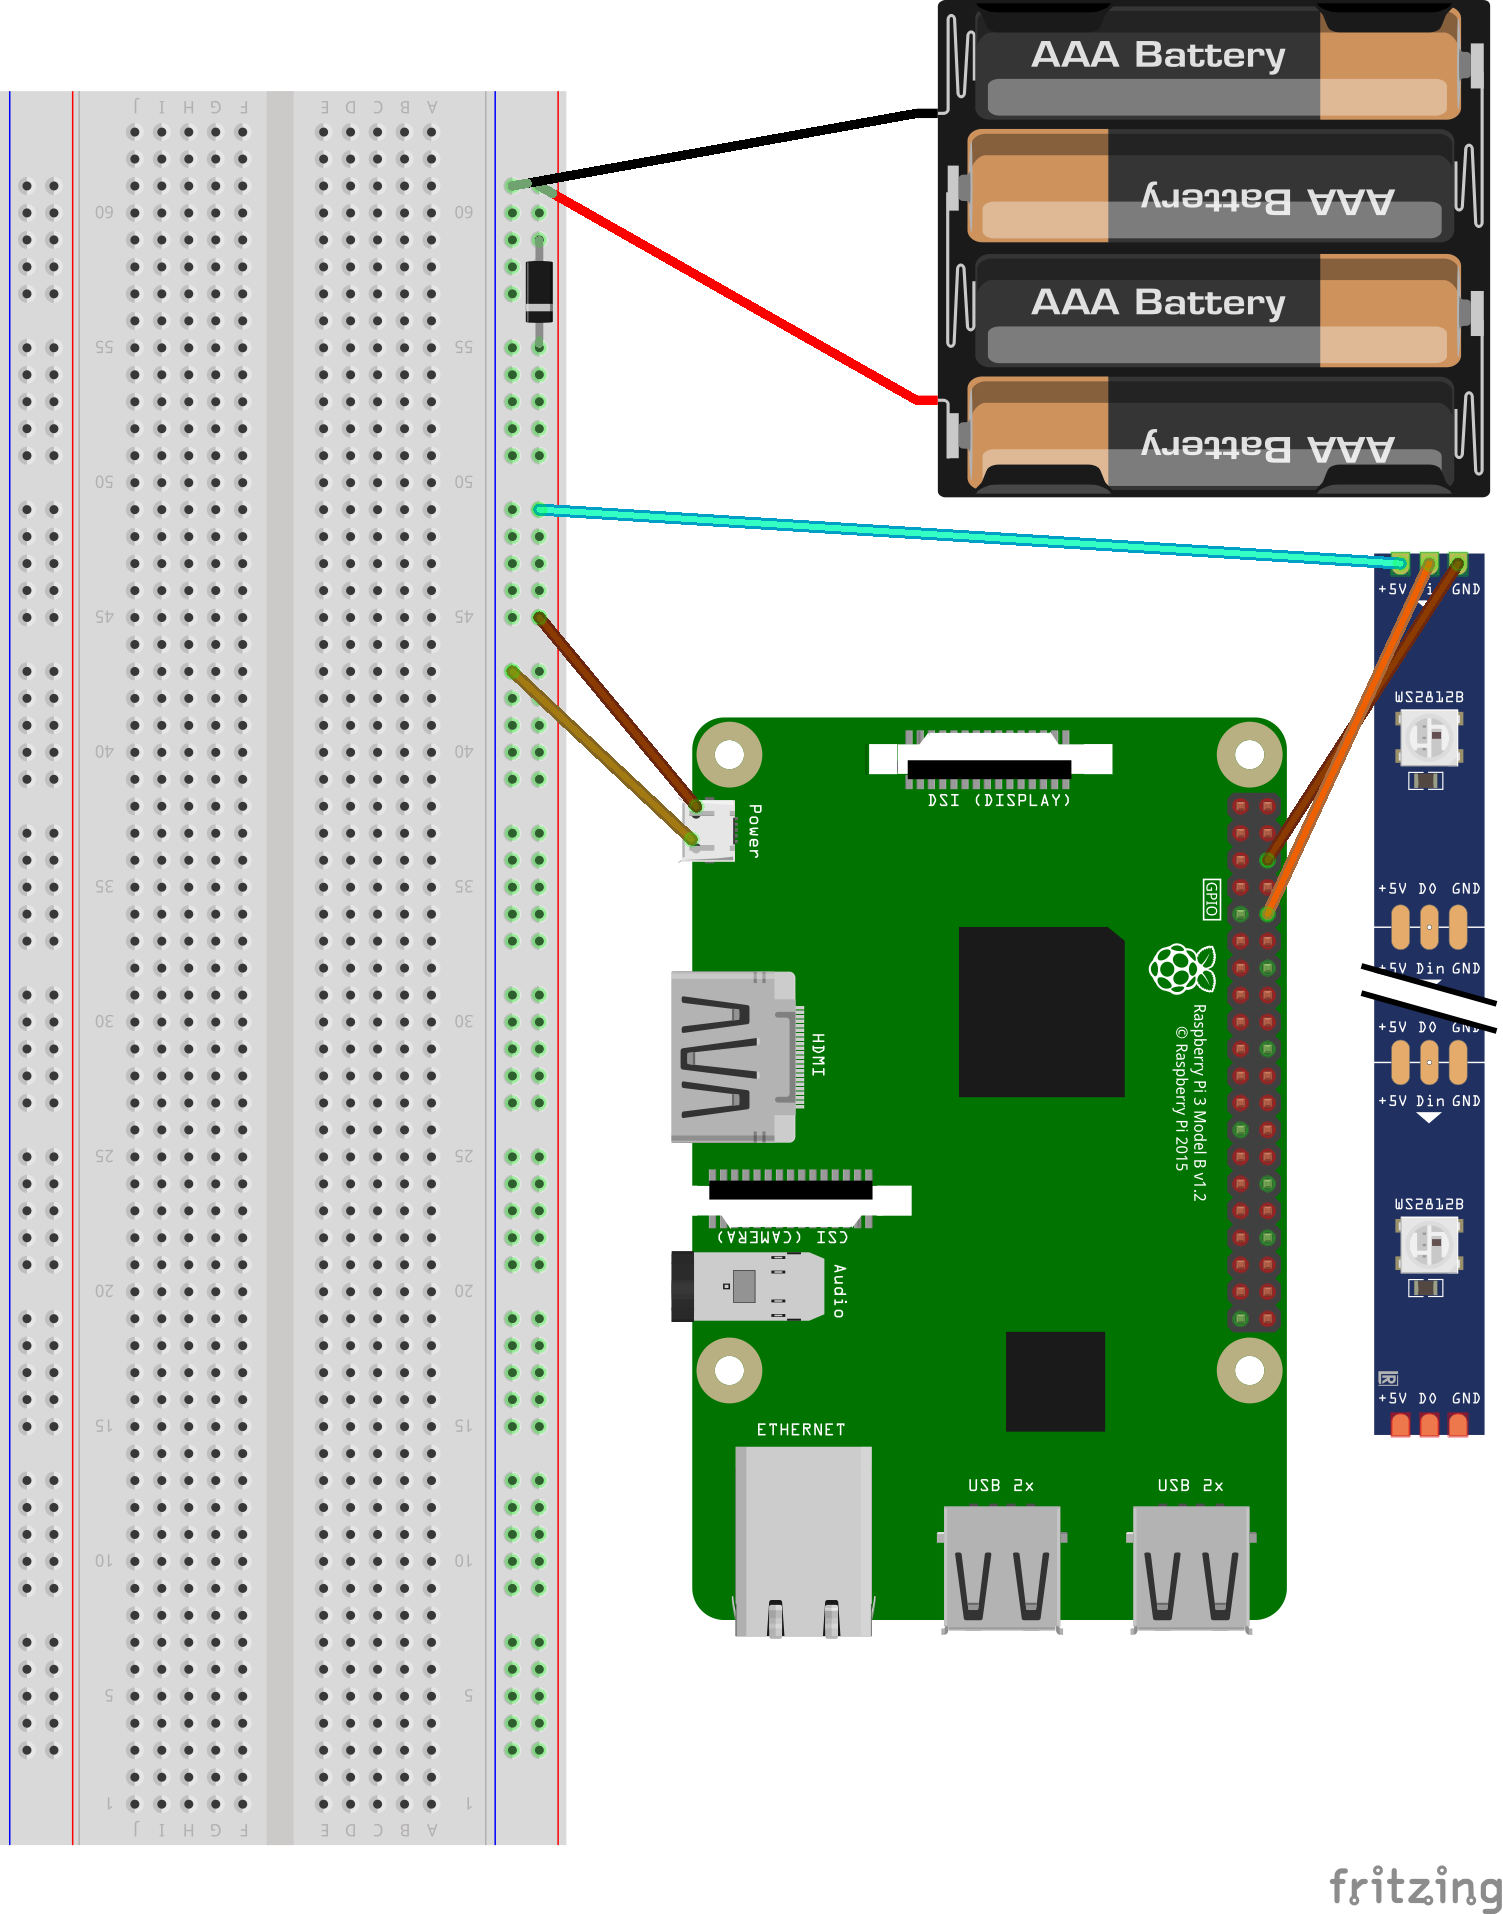
\includegraphics[height=0.4\textheight]{assets/images/practical/Итоговая архитектура программно-аппаратного комплекса.png}
  \caption{Итоговый макет программно-аппаратного комплекса}
  \label{img:all__schema}
\end{figure}

Согласно макету~\ref{img:all__schema} была собрана и протестирована работоспособность системы. На этом разработку аппаратной части комплекса можно считать завершённой.